\documentclass[xcolor={dvipsnames},aspectratio=169,10pt]{beamer}

% utility packages
\usepackage{multicol}
\usepackage{relsize}
\usepackage{amsthm}
\usepackage[spanish]{babel}
\usepackage{biblatex}
\usepackage{fontawesome}
\usepackage{pgfplots}
\usepackage{enumitem}
\usepackage{empheq}
\usepackage{xcolor}
\usepackage{epigraph}

% better text justifying
\usepackage{microtype}
% justify text inside list environment
% Ref: http://liam0205.me/2017/04/11/justifying-in-beamer-s-lists/
\usepackage{ragged2e}
\makeatletter
\patchcmd{\itemize}{\raggedright}{\justifying}{}{}
\patchcmd{\beamer@enum@}{\raggedright}{\justifying}{}{}
\patchcmd{\@@description}{\raggedright}{\justifying}{}{}
\makeatother

% math related packages
\usepackage{amsmath}
\usepackage[ruled,vlined]{algorithm2e}
\SetAlCapNameFnt{\scriptsize}
\SetAlCapFnt{\scriptsize}
\SetAlFnt{\scriptsize}

% figure related packages
\usepackage{graphicx}
\usepackage[scale=2]{ccicons}
\usepackage{tikz}
\usepackage{tikzpagenodes}
\usetikzlibrary{decorations.pathreplacing}
\usetikzlibrary{positioning}

% table related packages
\usepackage{array}
\usepackage{booktabs}
\usepackage{multirow}
\usepackage{colortbl}
\newcommand{\tabincell}[2]{\begin{tabular}{@{}#1@{}}#2\end{tabular}}

% hyperref setting
\hypersetup{
  unicode,
  psdextra,
  bookmarksnumbered=true,
  bookmarksopen=true,
  bookmarksopenlevel=3,
  bookmarksdepth=4,
  pdfcenterwindow=true,
  pdfstartview={Fit},
  pdfpagemode={FullScreen},
  pdfpagelayout={SinglePage},
}
\usepackage{bookmark}

% beamer theme
\usetheme{metropolis}
\metroset{block=fill,numbering=fraction}

% caption style
\usepackage{subcaption}
\setlength\abovecaptionskip{3pt}
\setbeamerfont{caption}{size=\scriptsize}
\renewcommand{\figurename}{Fig.}
\captionsetup{labelformat=empty,labelsep=none,textfont={bf,it}}

% Ref: https://github.com/gpoore/minted/blob/master/source/minted.dtx
\newenvironment{latexexample}
{\VerbatimEnvironment\begin{VerbatimOut}[gobble=3]{example.out}}{\end{VerbatimOut}%
  \begin{center}
    \begin{minipage}{0.47\linewidth}%
      \inputminted[resetmargins,fontsize=\scriptsize]{latex}{example.out}%
    \end{minipage}%
    \hspace{0.05\linewidth}%
    \begin{minipage}{0.47\linewidth}%
      \begin{framed}
        \setlength{\parindent}{2em}%
        \input{example.out}%
      \end{framed}
    \end{minipage}%
  \end{center}
}

\newenvironment{mathexample}
{\VerbatimEnvironment\begin{VerbatimOut}[gobble=3]{example.out}}{\end{VerbatimOut}%
  \begin{center}
    \begin{minipage}{0.47\linewidth}%
      \inputminted[resetmargins,fontsize=\scriptsize]{latex}{example.out}%
    \end{minipage}%
    \hspace{0.05\linewidth}%
    \begin{minipage}{0.47\linewidth}%
      \begin{framed}
        \[ \input{example.out} \]
      \end{framed}
    \end{minipage}%
  \end{center}
}

\newenvironment{mathexamples}
{\VerbatimEnvironment\begin{VerbatimOut}[gobble=3]{example.out}}{\end{VerbatimOut}%
  \begin{center}
    \begin{minipage}{0.47\linewidth}%
      \inputminted[resetmargins,fontsize=\scriptsize]{latex}{example.out}%
    \end{minipage}%
    \hspace{0.05\linewidth}%
    \begin{minipage}{0.47\linewidth}%
      \begin{framed}
        \directlua{
          local first = true
          for line in io.lines('example.out') do
          if first then
          first = false
          else
          tex.print('\\newline ')
          end
          tex.print('$' .. line .. '$')
          end
        }
      \end{framed}
    \end{minipage}%
  \end{center}
}

\title{Obtención de los Coeficientes de la forma canónica para la Elipse, hipérbolas y parábolas}
\subtitle{Determinación analítica de las cónicas}
\author{Grupo 12}
\date{December 05, 2023}
\titlegraphic{
  \begin{tikzpicture}[overlay, remember picture]
    \node[%
      above right=0.35cm and -0.2cm of current page footer area.south west,
      anchor=south west,
      inner sep=0pt] {%
      \usebeamerfont{footline}
    };
    % \node[%
    %   above left=0.35cm and 0cm of current page footer area.south east,
    %   anchor=south east,
    %   inner sep=0pt]{\qrcode[height=1.5cm]{https://github.com/axvg/presentaciones}};
  \end{tikzpicture}
}

\begin{document}

\maketitle%

\begin{frame}{Contenidos}
  \setbeamertemplate{section in toc}[sections numbered]
  \tableofcontents[hideallsubsections]
\end{frame}

\section{Introducción}

\begin{frame}{Formas cuadráticas}
    \frametitle{Formas cuadráticas}
    \begin{definition}
      Una forma cuadrática en n variables $x_{1}, x_{2}, . . . , x_{n}$ es una combinación lineal de los
      productos $x_{i} x_{j}$, esto es, una combinación lineal de cuadrados $x_{1}^2 , x_{2}^2 , . . . , x_{n}^2$ y
      términos $x_{1}x_{2}, x_{1}x_{3}, . . . , x_{1}x_{n}, x_{2}x_{3}, . . . , x_{2}x_{n}, . . . , x_{n-1}x_{n}$
    \end{definition}

  \begin{example}
    \begin{itemize}
        \item $q = x^2 - y^2 + 4xy$ y $q = x^2 + 3y^2 - 2xy$ son formas cuadráticas en $x$ y $y$.
        \item $q = -4x_{21} + x_{22}^2 + 4x_{23} + 6x_{1}x_{3}$ es una forma cuadrática en $x_{1}, x_{2}$ y $x_{3}$.
        \item La forma cuadrática general de $x_{1}, x_{2}, x_{3}$ es $a_{1}x_{21} + a_{2}x_{22}^2 + a_{3}x_{23} + a_{12}x_{1}x_{2} + a_{13}x_{1}x_{3} + a_{23}x_{2}x_{3}$.
    \end{itemize}
  \end{example}
\end{frame}

\begin{frame}{Formas cuadráticas}
  \frametitle{Formas cuadráticas}
  Las formas cuadráticas pueden ser escritas de la forma matricial $q(x) = x^{T}Ax$ donde $A$ es una matriz simétrica $n 
  \times n$ y $x$ es un vector columna $n \times 1$.

  La matriz $A$ es llamada la matriz de la forma cuadrática $q$.

  \begin{example}
    Supongamos que $q = x_1^2 - x_2^2 + 4x_1x_2$. Los coeficientes de $x_1^2$ y $x_2^2$ son 1 y -1, 
    respectivamente, por lo que colocamos estos, en orden, en las dos posiciones diagonales de una matriz A. 
    El coeficiente de $x_1x_2$ es 4, que dividimos equitativamente entre las posiciones (1, 2) y (2, 1), 
    colocando un 2 en cada lugar.
  \end{example}
\end{frame}

\begin{frame}{Formas cuadráticas}
  \frametitle{Formas cuadráticas}
  Así tenemos que:
  \begin{equation*}
    A = \begin{bmatrix}
      1 & 2 \\
      2 & -1
    \end{bmatrix}
  \end{equation*}
  y $x = \begin{bmatrix}
    x_1 \\
    x_2
  \end{bmatrix}$.
  Luego:
  \begin{equation*}
    q(x) = x^{T}Ax = \begin{bmatrix}
      x_1 & x_2
    \end{bmatrix}
    \begin{bmatrix}
      1 & 2 \\
      2 & -1
    \end{bmatrix}
    \begin{bmatrix}
      x_1 \\
      x_2
    \end{bmatrix}
    = x_1^2 - x_2^2 + 4x_1x_2
  \end{equation*}
\end{frame}

\section{Secciones Cónicas}

\begin{frame}{Secciones Cónicas}
  \frametitle{Secciones Cónicas}
  Se utiliza el término cónica para referirse a todas las curvas que surgen de las diversas intersecciones entre un cono y un plano. 
  Cuando dicho plano no cruza el vértice, se generan las cónicas específicas: parábola, elipse, hipérbola y circunferencia. 
  En este proyecto, nos enfocaremos únicamente en las tres primeras. 
  \begin{figure}
    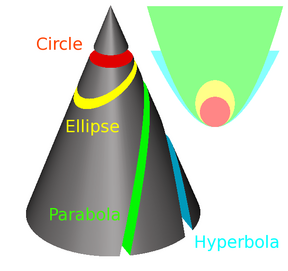
\includegraphics[width=0.5\textwidth, height=0.6\textheight, keepaspectratio]{images/conics.png}
    \caption{Las secciones cónicas: círculo, elipse, parábola y hipérbola}
  \end{figure}
\end{frame}

\begin{frame}{Forma General de las Secciones Cónicas}
  \begin{definition}
    Una sección cónica es el lugar en el plano cartesiano $\mathbb{R}^2$ de una ecuación de la forma
    \begin{equation*}
      ax^2 + bxy + cy^2 + dx + ey + f = 0. \tag{1}
    \end{equation*}
  \end{definition}
  Se puede demostrar que esta ecuación representa uno de los siguientes:
  \begin{enumerate}
    \item el conjunto vacío
    \item un solo punto
    \item una o dos rectas
    \item una elipse
    \item una hipérbola
    \item una parábola.
  \end{enumerate}
  La parte de segundo grado de (1), $q(x, y) = ax^2 + bxy + cy^2$ es una forma cuadrática. Esto determina el tipo de la cónica.
\end{frame}

\begin{frame}{Forma Matricial de las Secciones Cónicas}
  \frametitle{Forma Matricial de las Secciones Cónicas}
  Podemos escribir la ecuación en forma matricial:
  \begin{equation*}
    [x, y] \begin{bmatrix} a & b/2 \\ b/2 & c \end{bmatrix} \begin{bmatrix} x \\ y \end{bmatrix} + [d, e] \begin{bmatrix} x \\ y \end{bmatrix} + f = 0.
  \end{equation*}
  Escribimos $A = \begin{bmatrix} a & b/2 \\ b/2 & c \end{bmatrix}$. Sea $U = [u, v]$ una matriz ortogonal cuyos vectores de columna $u$ y $v$ son vectores propios de $A$ con valores propios $\lambda_1$ y $\lambda_2$. Aplicamos el cambio de variables
  \begin{equation*}
    x = \begin{bmatrix} x \\ y \end{bmatrix} = U \begin{bmatrix} u \\ v \end{bmatrix}
  \end{equation*}
  para diagonalizar la forma cuadrática $q(x, y)$ a la forma diagonal
  \begin{equation*}
    \lambda_1u^2 + \lambda_2v^2.
  \end{equation*}
\end{frame}

\begin{frame}{Transformación de Coordenadas}
  \frametitle{Transformación de Coordenadas}
  La base ortonormal \{u, v\} determina un nuevo conjunto de ejes de coordenadas con respecto a los cuales el lugar de la ecuación
  \begin{equation*}
    [x, y] A [x, y]^T + B [x, y]^T + f = 0
  \end{equation*}
  con B = [d, e] es el mismo que el lugar de la ecuación
  \begin{equation*}
    0 = [u, v] \text{diag} (\lambda_1, \lambda_2) [u, v]^T + (BU) [u, v]^T + f
  \end{equation*}
  por lo tanto
  \begin{equation*}
    \lambda_1 u^2 + \lambda_2 v^2 + [d, e] [u, v] [u, v]^T + f = 0 \tag{2}
  \end{equation*}
\end{frame}

\begin{frame}{Determinación del Tipo de Cónica}
  \frametitle{Determinación del Tipo de Cónica}
  Si la cónica determinada por (2) no es degenerada, es decir, no es un conjunto vacío, un punto, ni línea(s), entonces los signos de $\lambda_1$ y $\lambda_2$ determinan si es una parábola, una hipérbola o una elipse. La ecuación (1) representará
  \begin{itemize}
    \item una elipse si $\lambda_1\lambda_2 > 0$,
    \item una hipérbola si $\lambda_1\lambda_2 < 0$,
    \item una parábola si $\lambda_1\lambda_2 = 0$.
  \end{itemize}
\end{frame}

\begin{frame}{Parábola}
  \frametitle{Parábola}
  Una parábola es el lugar geométrico de un punto que se mueve en un plano de tal manera que su distancia a una recta fija, llamada directriz, situada en el mismo plano, 
  es siempre igual a su distancia a un punto fijo del plano, llamado foco, y que no pertenece a la recta.

  \begin{columns}
    \begin{column}{0.5\textwidth}
      \begin{figure}
        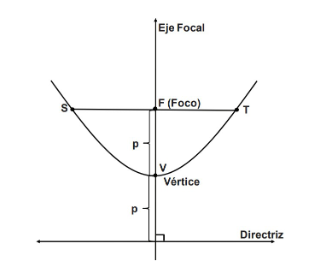
\includegraphics[width=\textwidth, height=0.6\textheight, keepaspectratio]{images/par1.png}
        \caption{Parábola y elementos}
      \end{figure}
    \end{column}
    \begin{column}{0.5\textwidth}
      \begin{itemize}\tiny
        \itemsep0em
        \item Eje Focal: es la recta que pasa por el foco y el vértice
        \item Foco (F): es el punto fijo que se indica en la definición
        \item Directriz: es la recta fija mencionada en la definición
        \item Vértice (V): es el punto donde el eje focal corta la parábola
        \item Distancia focal (p): es la distancia desde el vértice al foco y del vértice a la directriz.
        \item Lado Recto (ST): es el segmento perpendicular al eje focal, que pasa por el foco F, cuyos extremos son dos puntos de la parábola.
      \end{itemize}
    \end{column}
  \end{columns}
\end{frame}

\begin{frame}{Parámetros de la Parábola}
  \frametitle{Parámetros de la Parábola}

  \begin{table}[]
    \begin{tabular}{|c|c|c|}
    \hline
    & Parábola de eje vertical & Parábola de eje horizontal \\ \hline
    Ecuación General & $Ax^2 + Dx + Ey + F = 0$ & $Cy^2 + Dx + Ey + F = 0$ \\ 
    & $C = 0, A\neq0$ & $A = 0, C\neq 0$ \\ \hline
    Ecuación canónica & $(x-h)^2 = 4p(y-k)$ & $(y-k)^2 = 4p(x-h)$ \\ \hline
    Coordenadas del Vértice & $(h, k)$ & $(h, k)$ \\ \hline
    Coordenadas del Foco & $(h, k+p)$ & $(h+p, k)$ \\ \hline
    Ecuación de la Directriz & $y=k-p$ & $x=h-p$ \\ \hline
    Ecuación del eje focal & $x=h$ & $y=k$ \\ \hline
    \end{tabular}
  \end{table}
\end{frame}

\begin{frame}{Elipse}
  \frametitle{Elipse}
    Una elipse es el conjunto de todos los puntos en un plano cuya distancia a dos puntos fijos en el plano tienen una suma constante. 
    Los puntos fijos son los focos de la elipse. La recta que une los focos es el eje focal. El punto sobre el eje focal que está en el 
    punto medio entre los dos focos es el centro. Los puntos donde la elipse interseca a su eje son los vértices de la elipse.
  \begin{columns}
    \begin{column}{0.5\textwidth}
      \begin{tikzpicture}[dot/.style={draw,fill,circle,inner sep=1pt}]
        \def\a{4}
        \def\b{3}
        \def\angle{-45}
        \draw (0,0) ellipse ({\a} and {\b});
        \draw (-\a,0) coordinate[label={left:$A$}] (A)
          -- (\a,0) coordinate[label={right:$B$}] (B);
        \draw (0,-\b) coordinate[label={below:$D$}] (D)
          -- (0,\b) coordinate[label={above:$C$}] (C);
        \coordinate[label={below right:$S(p,q)$}] (O) at (0,0);
        \node[dot,label={below:$F_1$}] (F1) at ({-sqrt(\a*\a-\b*\b)},0) {};
        \node[dot,label={below:$F_2$}] (F2) at ({+sqrt(\a*\a-\b*\b)},0) {};
        \node[dot,label={\angle:$X$}] (X) at (\angle:{\a} and {\b}) {};
        \draw (F1) -- (X) (X) -- (F2);
        \draw[decorate,decoration=brace,draw=red] (C) -- (O);
      \end{tikzpicture}
    \end{column}
    \begin{column}{0.5\textwidth}
      \begin{itemize}
        \item Eje Mayor: es el segmento que pasa por los focos y los vértices de la elipse
        \item Eje Menor: es el segmento perpendicular al eje mayor en el centro de la elipse
        \item Focos (F): son los dos puntos fijos en la definición de la elipse
        \item Vértices (V): son los puntos donde el eje mayor corta la elipse
      \end{itemize}
    \end{column}
  \end{columns}
\end{frame}

\begin{frame}{Elementos de la Hipérbola}
  \frametitle{Elementos de la Hipérbola}
  \begin{table}[]
    \begin{tabular}{|c|c|c|}
    \hline
    & Hipérbola de eje horizontal & Hipérbola de eje vertical \\ \hline
    Ecuación General & $Ax^2 - Cy^2 + Dx + Ey + F = 0$ & $-Ax^2 + Cy^2 + Dx + Ey + F = 0$ \\ 
    & Con $A$ y $C$ no ambas cero, distinto valor numérico y signos contrarios. & Con $A$ y $C$ no ambas cero, distinto valor numérico y signos contrarios. \\ 
    & $B = 0$ (Sin rotación de ejes) & $B = 0$ (Sin rotación de ejes) \\ \hline
    Ecuación canónica & $(x-h)^2/a^2 - (y-k)^2/b^2 = 1$ & $(y-k)^2/b^2 - (x-h)^2/a^2 = 1$ \\ \hline
    Localización de los focos & $(h \pm c, k)$ & $(h, k \pm c)$ \\ \hline
    Localización de los vértices & $(h \pm a, k)$ & $(h, k \pm a)$ \\ \hline
    Ecuación del eje focal & $y=k$ & $x=h$ \\ \hline
    Semieje focal & $a$ & $a$ \\ \hline
    Semieje conjugado & $b$ & $b$ \\ \hline
    Longitud focal & $c$ & $c$ \\ \hline
    Relación pitagórica & $c^2 = a^2 + b^2$ & $c^2 = a^2 + b^2$ \\ \hline
    Ecuación de las asinfotas & $y = k \pm \frac{b}{a}(x - h)$ & $x = h \pm \frac{a}{b}(y - k)$ \\ \hline
    \end{tabular}
  \end{table}
\end{frame}

\begin{frame}{Hipérbola}
  \frametitle{Hipérbola}
    Una hipérbola es el conjunto de todos los puntos en un plano cuya diferencia de distancias a dos puntos fijos en el plano es una constante. 
    Los puntos fijos son los focos de la hipérbola. La recta que une los focos es el eje focal. El punto sobre el eje focal que está en el 
    punto medio entre los dos focos es el centro. Los puntos donde la hipérbola interseca a su eje son los vértices de la hipérbola.
  \begin{columns}
    \begin{column}{0.5\textwidth}
      \begin{figure}
        \begin{tikzpicture}[dot/.style={draw,fill,circle,inner sep=1pt}]
          \def\a{4}
          \def\b{3}
          \def\angle{-45}
          \draw plot[domain=-2:2] ({\a*cosh(\x)}, {\b*sinh(\x)});
          \draw plot[domain=-2:2] ({-\a*cosh(\x)}, {\b*sinh(\x)});
          \draw (-\a,0) coordinate[label={left:$A$}] (A)
            -- (\a,0) coordinate[label={right:$B$}] (B);
          \draw (0,-\b) coordinate[label={below:$D$}] (D)
            -- (0,\b) coordinate[label={above:$C$}] (C);
          \coordinate[label={below right:$S(p,q)$}] (O) at (0,0);
          \node[dot,label={below:$F_1$}] (F1) at ({-sqrt(\a*\a+\b*\b)},0) {};
          \node[dot,label={below:$F_2$}] (F2) at ({+sqrt(\a*\a+\b*\b)},0) {};
          \node[dot,label={\angle:$X$}] (X) at (\angle:{\a} and {\b}) {};
          \draw (F1) -- (X) (X) -- (F2);
          \draw[decorate,decoration=brace,draw=red] (C) -- (O);
        \end{tikzpicture}
        \caption{Hipérbola y sus elementos}
      \end{figure}
    \end{column}
    \begin{column}{0.5\textwidth}
      \begin{itemize}
        \item Eje Transverso: es el segmento que pasa por los focos y los vértices de la hipérbola
        \item Eje Conjugado: es el segmento perpendicular al eje transverso en el centro de la hipérbola
        \item Focos (F): son los dos puntos fijos en la definición de la hipérbola
        \item Vértices (V): son los puntos donde el eje transverso corta la hipérbola
      \end{itemize}
    \end{column}
  \end{columns}
\end{frame}

\begin{frame}{Elementos de la Hipérbola}
  \frametitle{Elementos de la Hipérbola}
  \begin{table}[]
    \begin{tabular}{|c|c|c|}
    \hline
    & Hipérbola de eje horizontal & Hipérbola de eje vertical \\ \hline
    Ecuación General & $Ax^2 - Cy^2 + Dx + Ey + F = 0$ & $-Ax^2 + Cy^2 + Dx + Ey + F = 0$ \\ 
    & Con $A$ y $C$ no ambas cero, distinto valor numérico y signos contrarios. & Con $A$ y $C$ no ambas cero, distinto valor numérico y signos contrarios. \\ 
    & $B = 0$ (Sin rotación de ejes) & $B = 0$ (Sin rotación de ejes) \\ \hline
    Ecuación canónica & $(x-h)^2/a^2 - (y-k)^2/b^2 = 1$ & $(y-k)^2/b^2 - (x-h)^2/a^2 = 1$ \\ \hline
    Localización de los focos & $(h \pm c, k)$ & $(h, k \pm c)$ \\ \hline
    Localización de los vértices & $(h \pm a, k)$ & $(h, k \pm a)$ \\ \hline
    Ecuación del eje focal & $y=k$ & $x=h$ \\ \hline
    Semieje focal & $a$ & $a$ \\ \hline
    Semieje conjugado & $b$ & $b$ \\ \hline
    Longitud focal & $c$ & $c$ \\ \hline
    Relación pitagórica & $c^2 = a^2 + b^2$ & $c^2 = a^2 + b^2$ \\ \hline
    Ecuación de las asinfotas & $y = k \pm \frac{b}{a}(x - h)$ & $x = h \pm \frac{a}{b}(y - k)$ \\ \hline
    \end{tabular}
  \end{table}
\end{frame}

\begin{frame}{Bibliografia}
  \begin{itemize}
    \item \faGlobe\, Applications of Linear Algebra in Various Fields (Part-1): \url{https://www.researchgate.net/publication/356818396_Applications_of_Linear_Algebra_in_Various_Fields_Part-1}
    \item \faBook\, Álgebra lineal y geometría cartesiana - Juan de Burgos Román
    \item \faBook\, Practical Linear Algebra: A Geometry Toolbox - Gerald Farin, Dianne Hansford
  \end{itemize}
\end{frame}

\begin{frame}[standout]
  Gracias \\
\end{frame}

\end{document}